\documentclass[tikz,border=10pt]{standalone}
\usetikzlibrary{angles}

\begin{document}
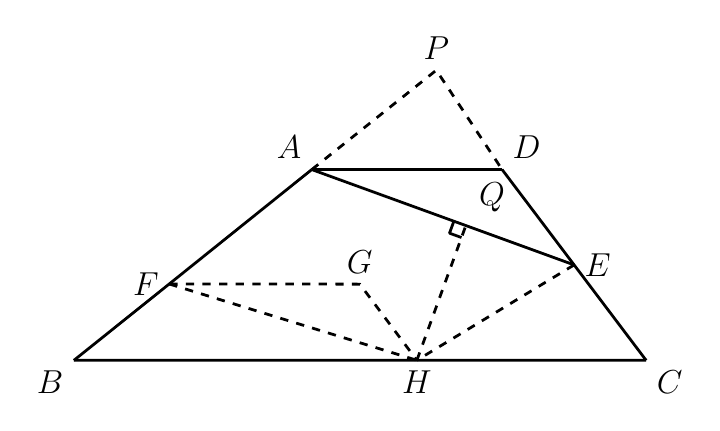
\begin{tikzpicture}[line width=1.0pt, line join=round]
\coordinate (A) at (-0.612,0.613);
\coordinate (B) at (-3.633,-1.810);
\coordinate (C) at (3.635,-1.810);
\coordinate (D) at (1.804,0.615);
\coordinate (E) at (2.720,-0.598);
\coordinate (G) at (-0.002,-0.842);
\coordinate (H) at (0.723,-1.809);
\coordinate (P) at (0.970,1.875);
\coordinate (Q) at (1.345,-0.098);




\coordinate (F) at (-2.422,-0.840);



\draw (B) -- (H) -- (C);
\draw (B) -- (F) -- (A);


\draw (A) -- (D);
\draw (C) -- (E) -- (D);


\draw (A) -- (Q) -- (E);


\draw[dashed] (A) -- (P) -- (D);


\draw[dashed] (F) -- (G) -- (H);
\draw[dashed] (F) -- (H);
\draw[dashed] (E) -- (H);
\draw[dashed] (H) -- (Q);


\draw pic[draw, angle radius=0.162cm] {right angle=A--Q--H};


\node[font=\fontsize{11.5}{13.7}\selectfont, below left] at (B) {$B$};
\node[font=\fontsize{11.5}{13.7}\selectfont, below] at (H) {$H$};
\node[font=\fontsize{11.5}{13.7}\selectfont, below right] at (C) {$C$};
\node[font=\fontsize{11.5}{13.7}\selectfont, above left] at (A) {$A$};
\node[font=\fontsize{11.5}{13.7}\selectfont, left] at (F) {$F$};
\node[font=\fontsize{11.5}{13.7}\selectfont, above] at (G) {$G$};
\node[font=\fontsize{11.5}{13.7}\selectfont, above right] at (D) {$D$};
\node[font=\fontsize{11.5}{13.7}\selectfont, right] at (E) {$E$};

\node[font=\fontsize{11.5}{13.7}\selectfont, above right, xshift=1pt, yshift=1pt] at (Q) {$Q$};
\node[font=\fontsize{11.5}{13.7}\selectfont, above] at (P) {$P$};
\end{tikzpicture}
\end{document}
